%% V1.0
%% by Gabriel Garcia, gabrcg@gmail.com
%% This is a template for Udacity projects using IEEEtran.cls

%% Be Udacious!

\documentclass[10pt,journal,compsoc]{IEEEtran}

\usepackage[pdftex]{graphicx}
\usepackage{cite}
\hyphenation{op-tical net-works semi-conduc-tor}
\usepackage{hyperref}

\begin{document}

\title{Map My World}

\author{Jeremy Hale}

\markboth{SLAM, Robotics Nanodegree Program, Udacity}%
{}
\IEEEtitleabstractindextext{%

\begin{abstract}
The Udacity Robotics Nanodegree project Map My World is a simluation of a small robot mapping two different environments. The robot uses a RGBD camera and a laser scanner with the RTAB-Map method of SLAM (simultaenous localization and mapping) to create a map of the environments. ROS and Gazebo/RViz are the main tools employed. The robot successfully maps the provided "Kitchen \& Dining" world, but difficulty in finding loop closures was found with the student "Back Alley" world.
\end{abstract}

% Note that keywords are not normally used for peerreview papers.
\begin{IEEEkeywords}
Robot, IEEEtran, Udacity, \LaTeX, Localization.
\end{IEEEkeywords}}


\maketitle
\IEEEdisplaynontitleabstractindextext
\IEEEpeerreviewmaketitle
\section{Introduction}
\label{sec:introduction}

\IEEEPARstart{T}{his} project demonstrates the use of SLAM in simulation using ROS and specifically the RTAB-Map implementation of SLAM. SLAM is a technique to solve the problem of localization while building a map from sensor inputs. In this simulation, a small two-wheel robot with RBGD camera and laser scanner is manually navigated around an environment. During navigation, the robot uses its sensor inputs to build a map of the environment.

The problem of mapping applies to many different situations as a robot may commonly find itself in an environment for which it does not have a map a priori. Even if a map were to exist, most environments in the world are not static. In homes and offices, for example, furniture or other significant objects or obstructions may be moved and would differ from prior maps.

\section{Background}
Any robot that needs to navigate autonomously needs a map in order to plan a route from the origin to the destination. This map could be a "world" map and the robot could use GPS to navigate, but for any indoor application or an outdoor application where obstructions are likely to move, a map will either not exist or not be sufficiently helpful for navigation. Therefore, the robot must determine the map itself and also determine its location relative to this map. This technique of determining the map and the robot pose is referred to as SLAM, or Simultaneous Localization and Mapping.


During the classroom work for this project, several varieties of SLAM were discussed such as FastSLAM and GraphSLAM. FastSLAM uses a particle filter to estimate the posterior probability of the trajectory and a low-dimensional extended Kalman filter to estimate the map. FastSLAM requires known landmark positions. Grid-based FastSLAM obviates the need for known landmarks by using Occupancy Grid Mapping for solving the mapping problem.

The algorithm used in this project is RTAB-Map (real-time appearance-based) which is based on GraphSLAM. GraphSLAM is regarded as more accurate than the particle-based approach of FastSLAM because it solves the Full SLAM problem of solving the full trajectory and not just the current pose. RTAB-Map, in specific, is composed of a front-end and back-end. The front-end includes sensor data and odometry as well an algorithm to detecting loop closures. The back-end is concerned with graph optimization and map generation. The loop closure algorithm determines if the robot has returned to a previous location based on similarity of the sensor data and odometry.

For the robot in discussion here, a 2D map is sufficient, because our robot moves only in 2D space. However, for airborne robots like drones a 3D map is necessary because they move in three dimensions.


\section{Model Configuration}
The robot was based on the Udacity robot from the "Where am I?" project. It was a small box-shaped chassis with 2 driven-wheels on the sides and 2 stabilizing wheels fore and aft. The robot has a Hokuyo laser scanner and a camera attached on the front. In the previous project, the camera was a simple RGB camera. This was changed to an RGBD camera to satisfy the project requirements.

\begin{figure}[thpb]
    \centering
    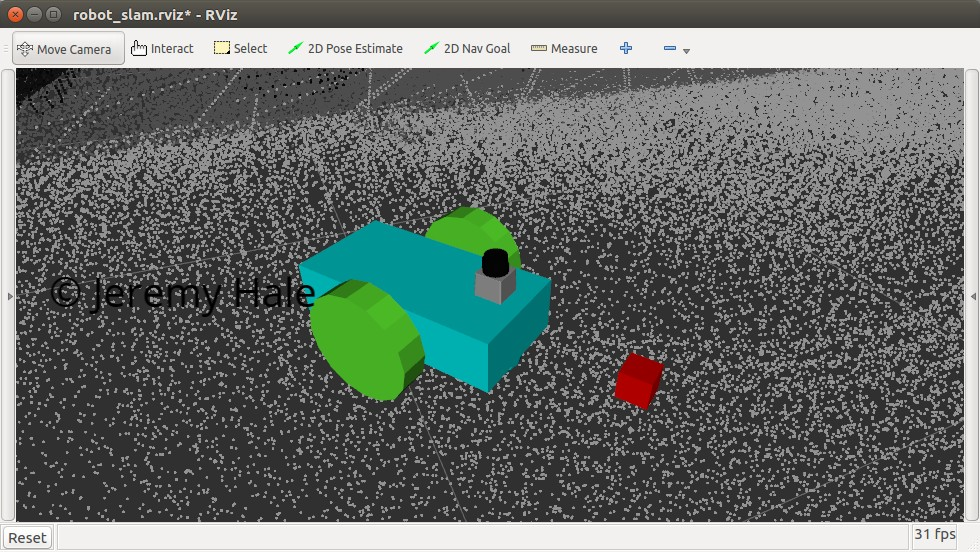
\includegraphics[width=\linewidth]{robot}
    \caption{Robot}
    \label{fig:robot}
\end{figure}

\begin{figure}[thpb]
    \centering
    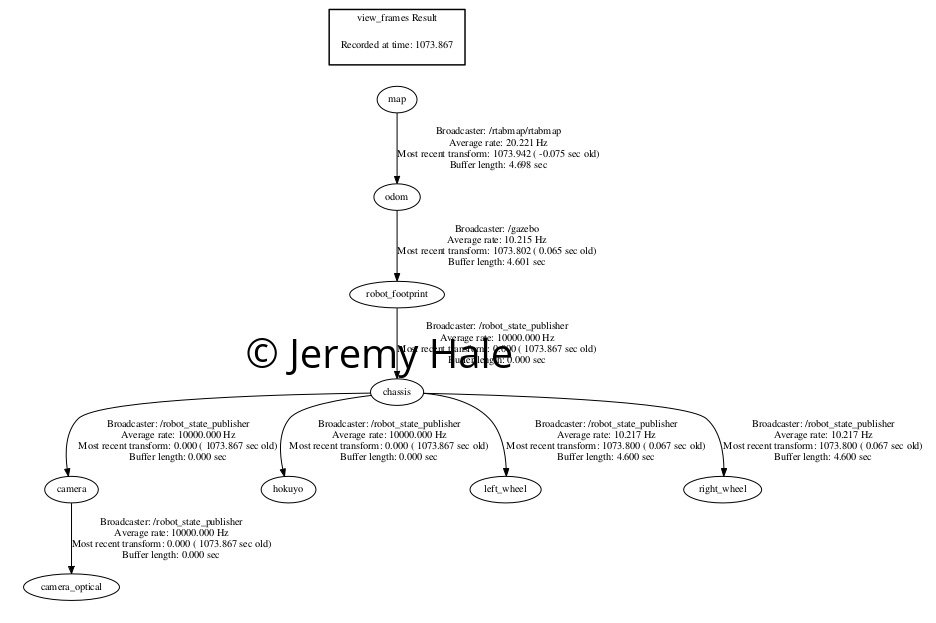
\includegraphics[width=\linewidth]{frames}
    \caption{TF Frames}
    \label{fig:frames}
\end{figure}

\section{World Creation}
The personal "world" is supposed to be a back alley. There is a large brick wall, a pickup truck, a dumpster and a fire hydrant.

\begin{figure}[thpb]
    \centering
    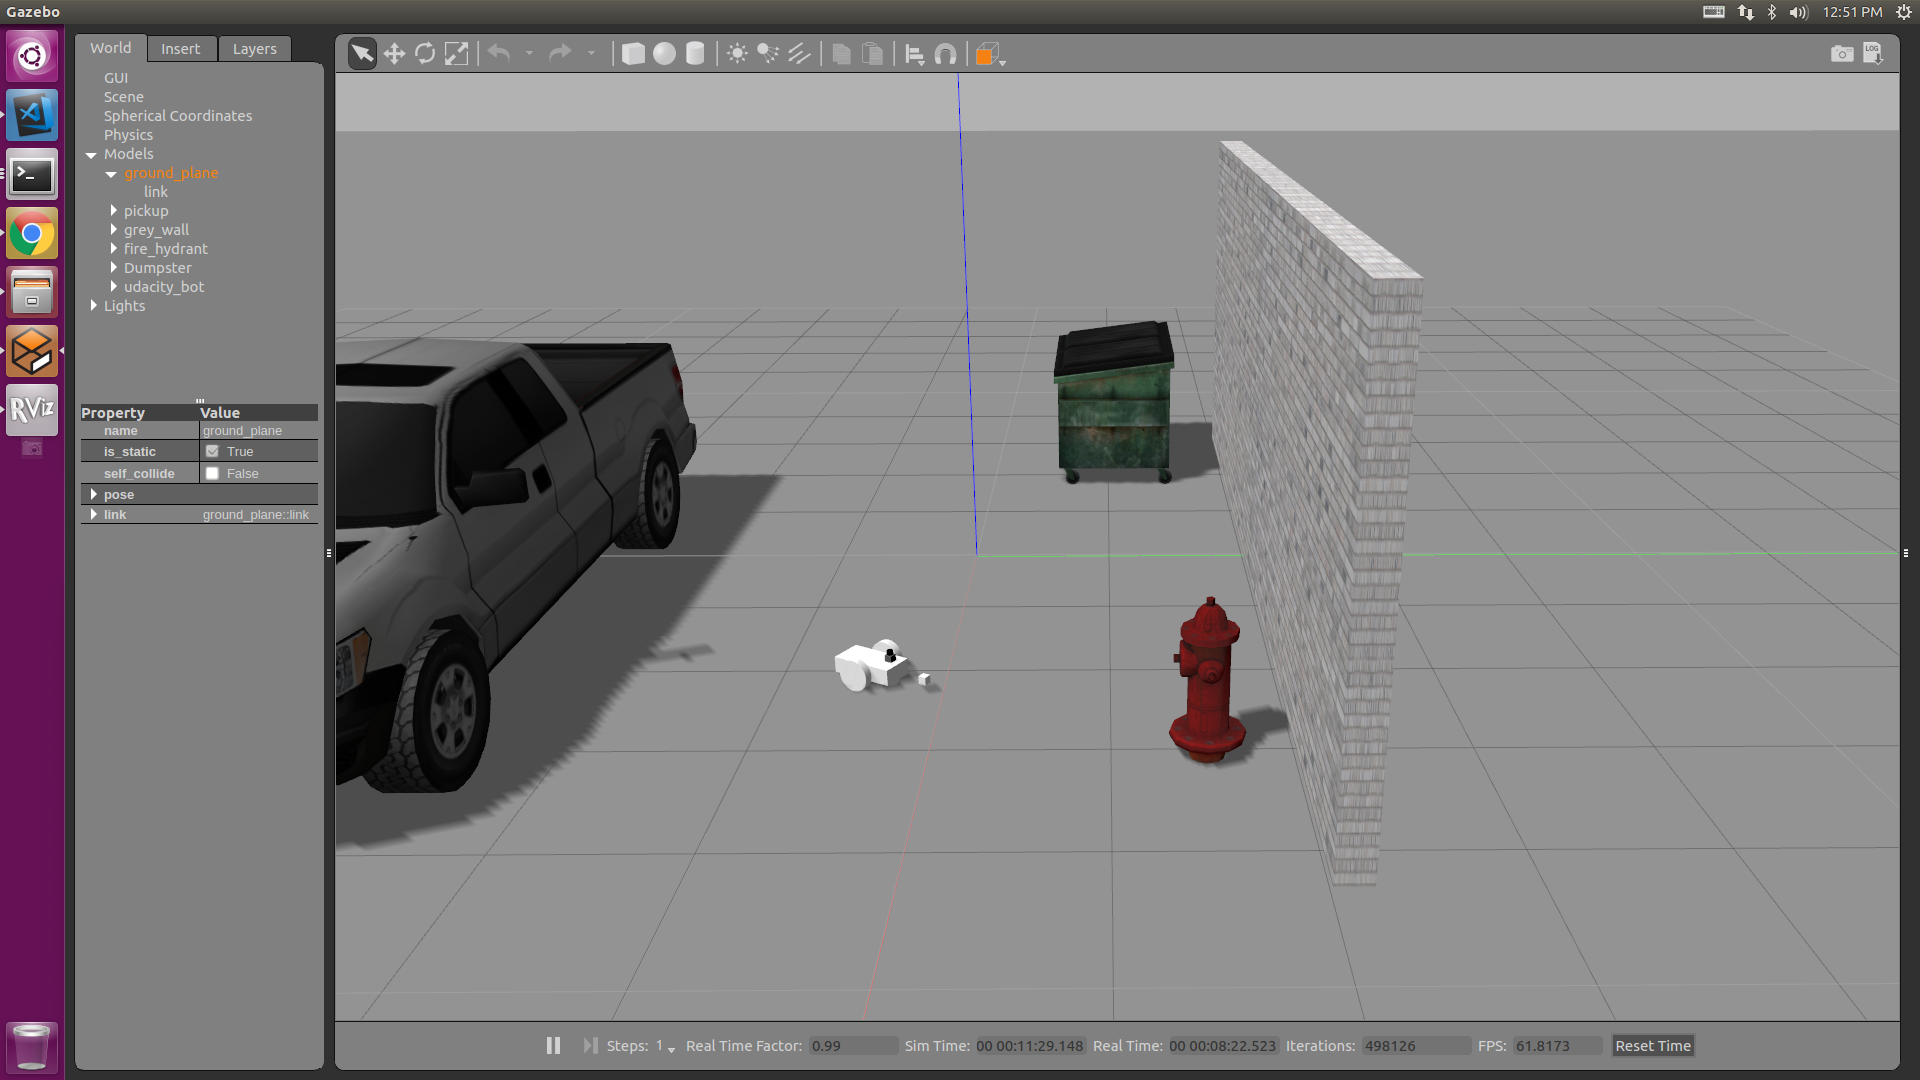
\includegraphics[width=\linewidth]{alley_no_cone}
    \caption{Alley}
    \label{fig:alley}
\end{figure}

\section{Results}

The databases are available at

"Kitchen and Dining":
\url{https://drive.google.com/open?id=1DOQL2NfoW7_gt6mpnxwsNIt73ukykCSr}

"Back Alley":
\url{https://drive.google.com/open?id=1ZlF_6YFfxB6r0OdK1i7AOHycmMz3a-Cl}


\subsection{Kitchen \& Dining}

The occupancy and 3D maps for the "Kitchen and Dining" world are shown below. There are also images showing the 3 closures.

\begin{figure}[thpb]
    \centering
    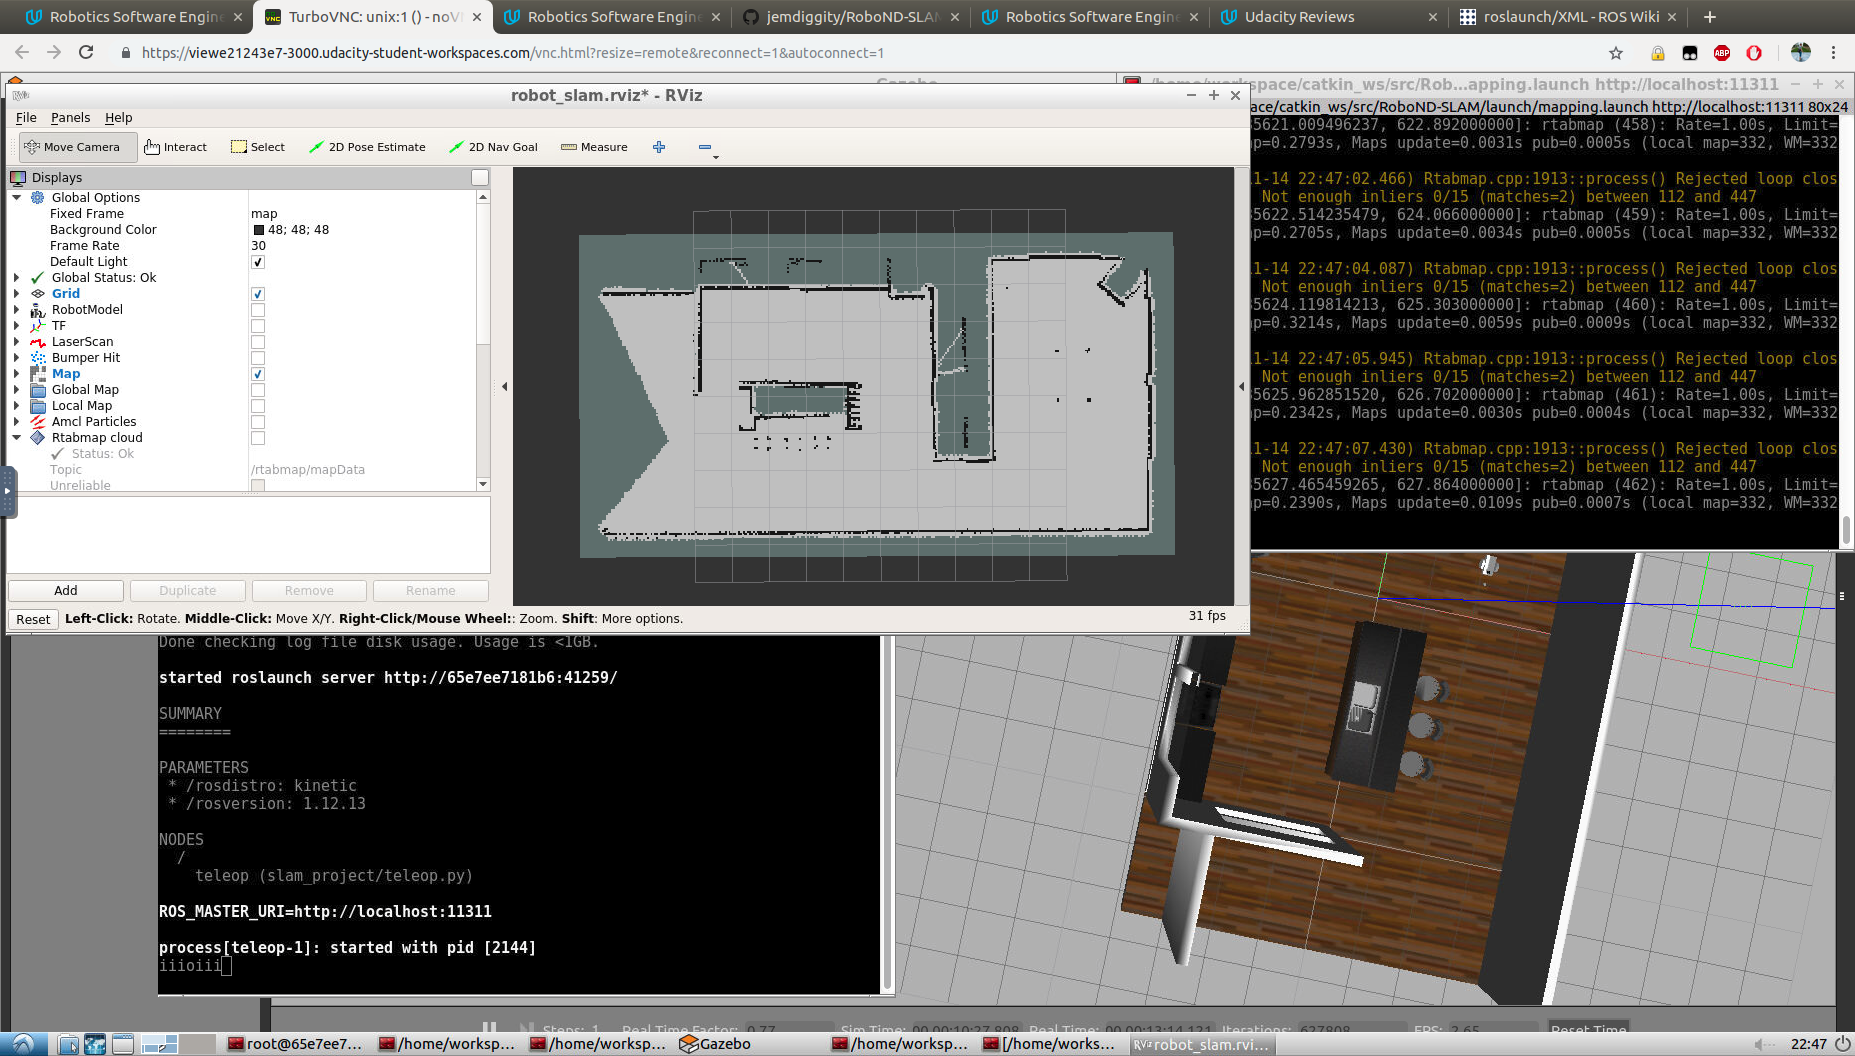
\includegraphics[width=\linewidth]{dining_map}
    \caption{Kitchen \& Dining Occupancy Map}
    \label{fig:dining_2d}
\end{figure}

\begin{figure}
    \centering
    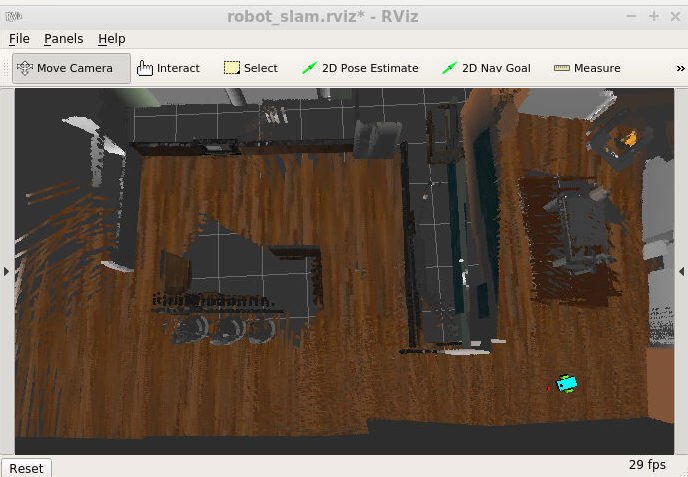
\includegraphics[width=\linewidth]{workspace_benchmark_crop}
    \caption{Kitchen \& Dining 3D Map}
    \label{fig:dining_3d}
\end{figure}

\begin{figure}
    \centering
    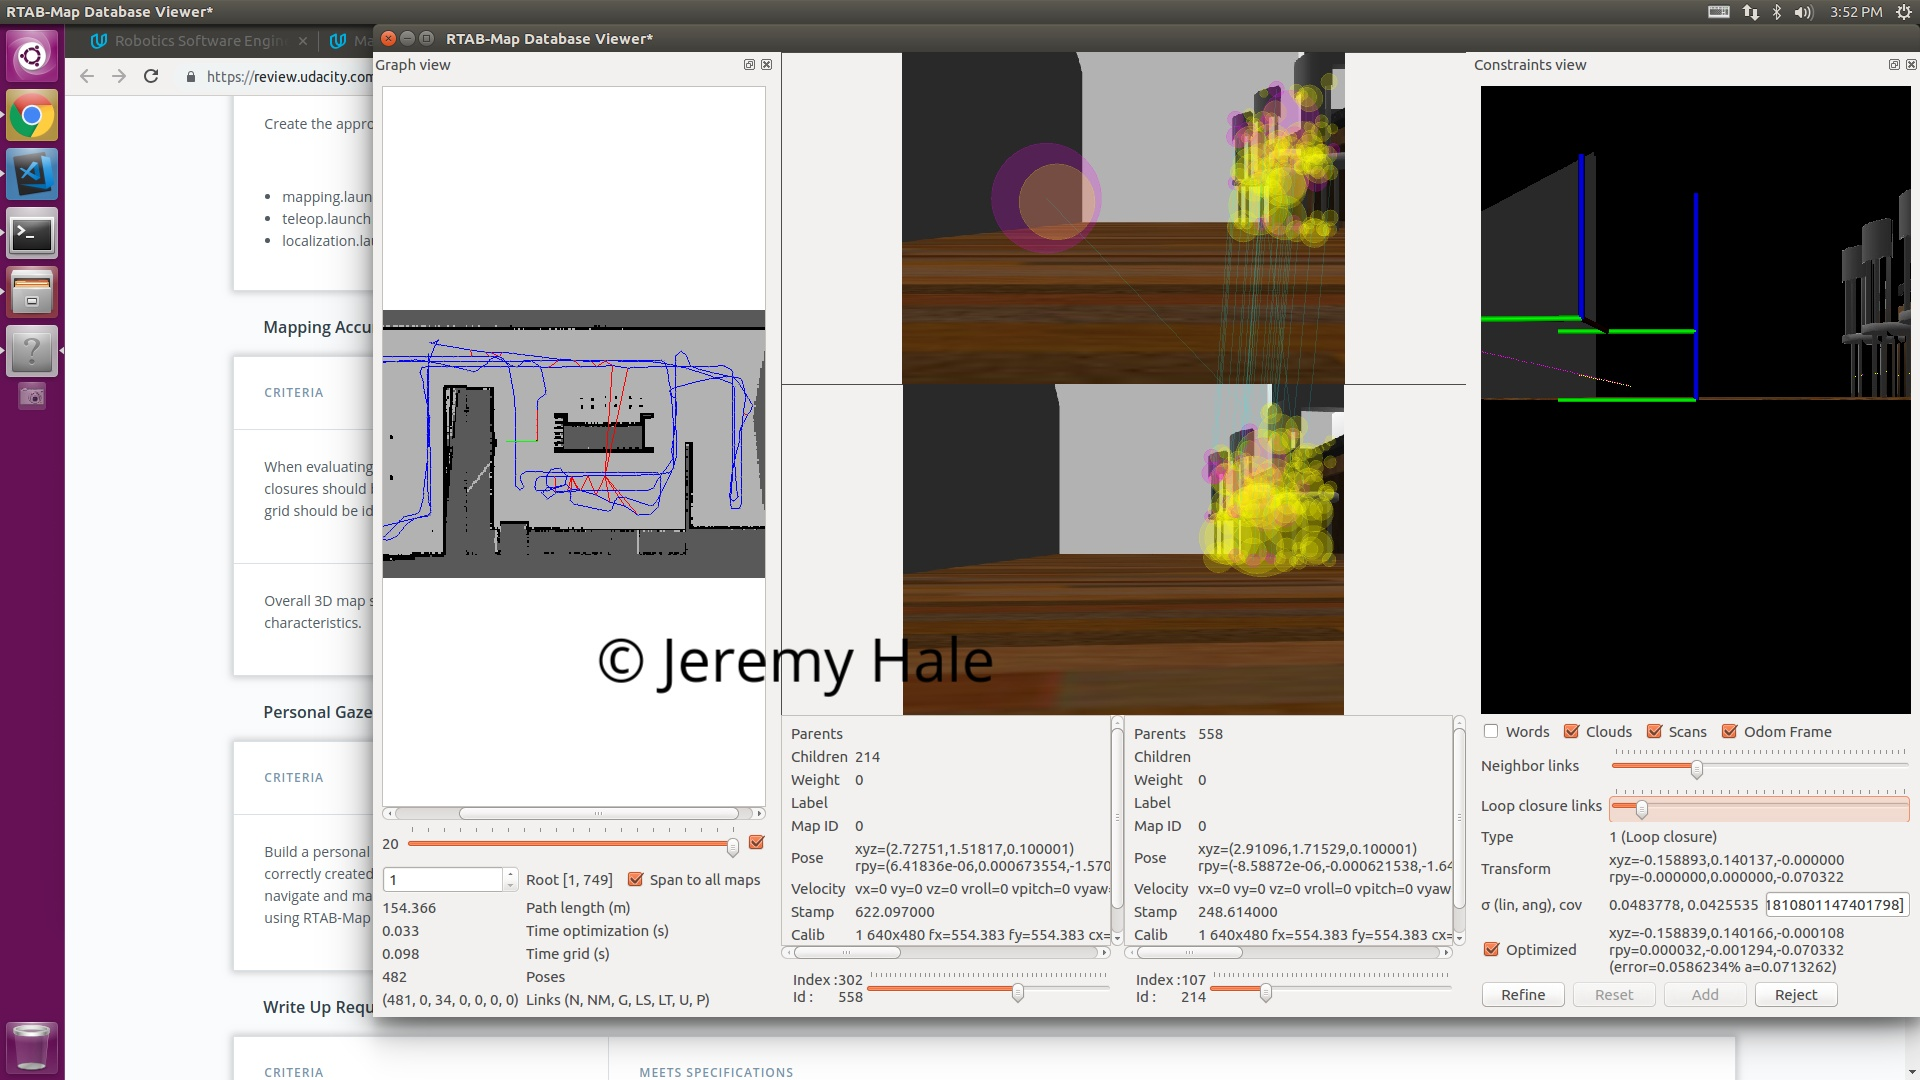
\includegraphics[width=\linewidth]{closure_1}
    \caption{Udacity World Closure}
    \label{fig:closure 1}
\end{figure}

\begin{figure}
    \centering
    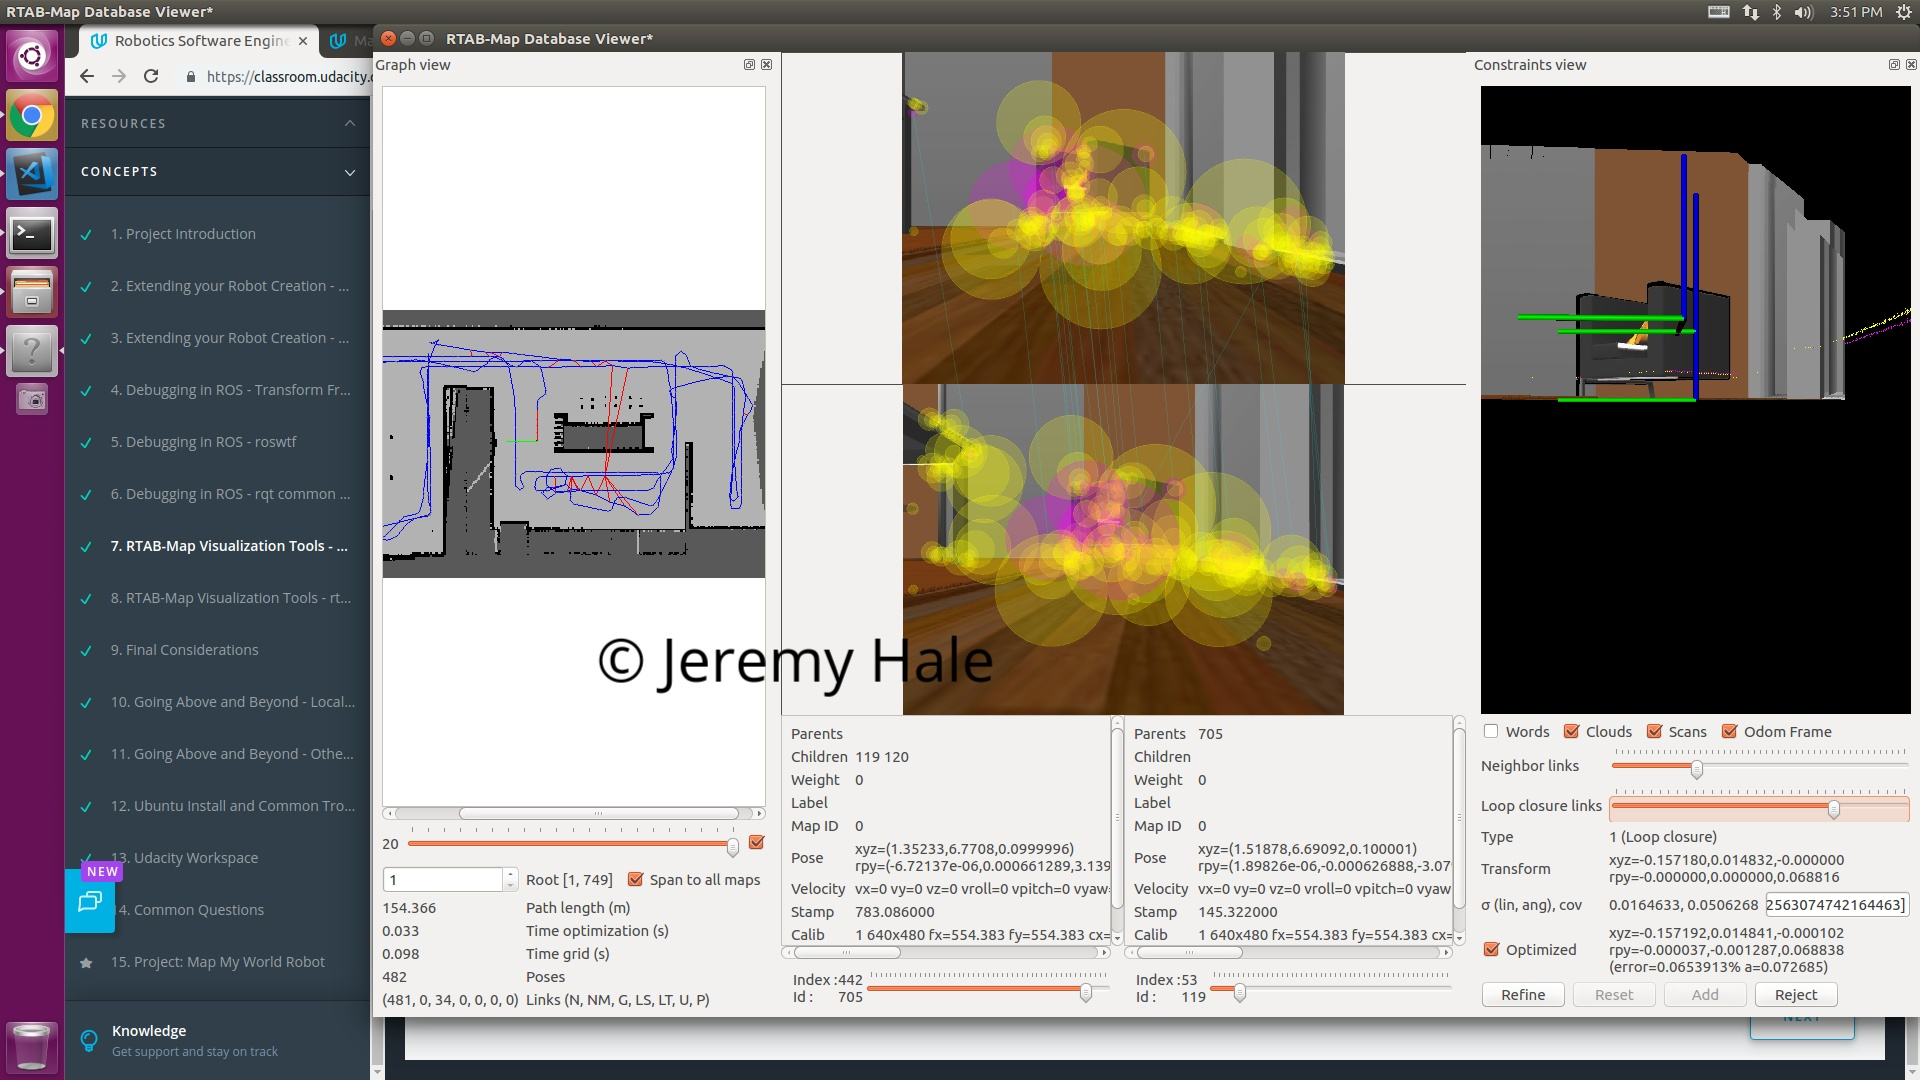
\includegraphics[width=\linewidth]{closure_2}
    \caption{Udacity World Closure}
    \label{fig:closure 2}
\end{figure}

\begin{figure}
    \centering
    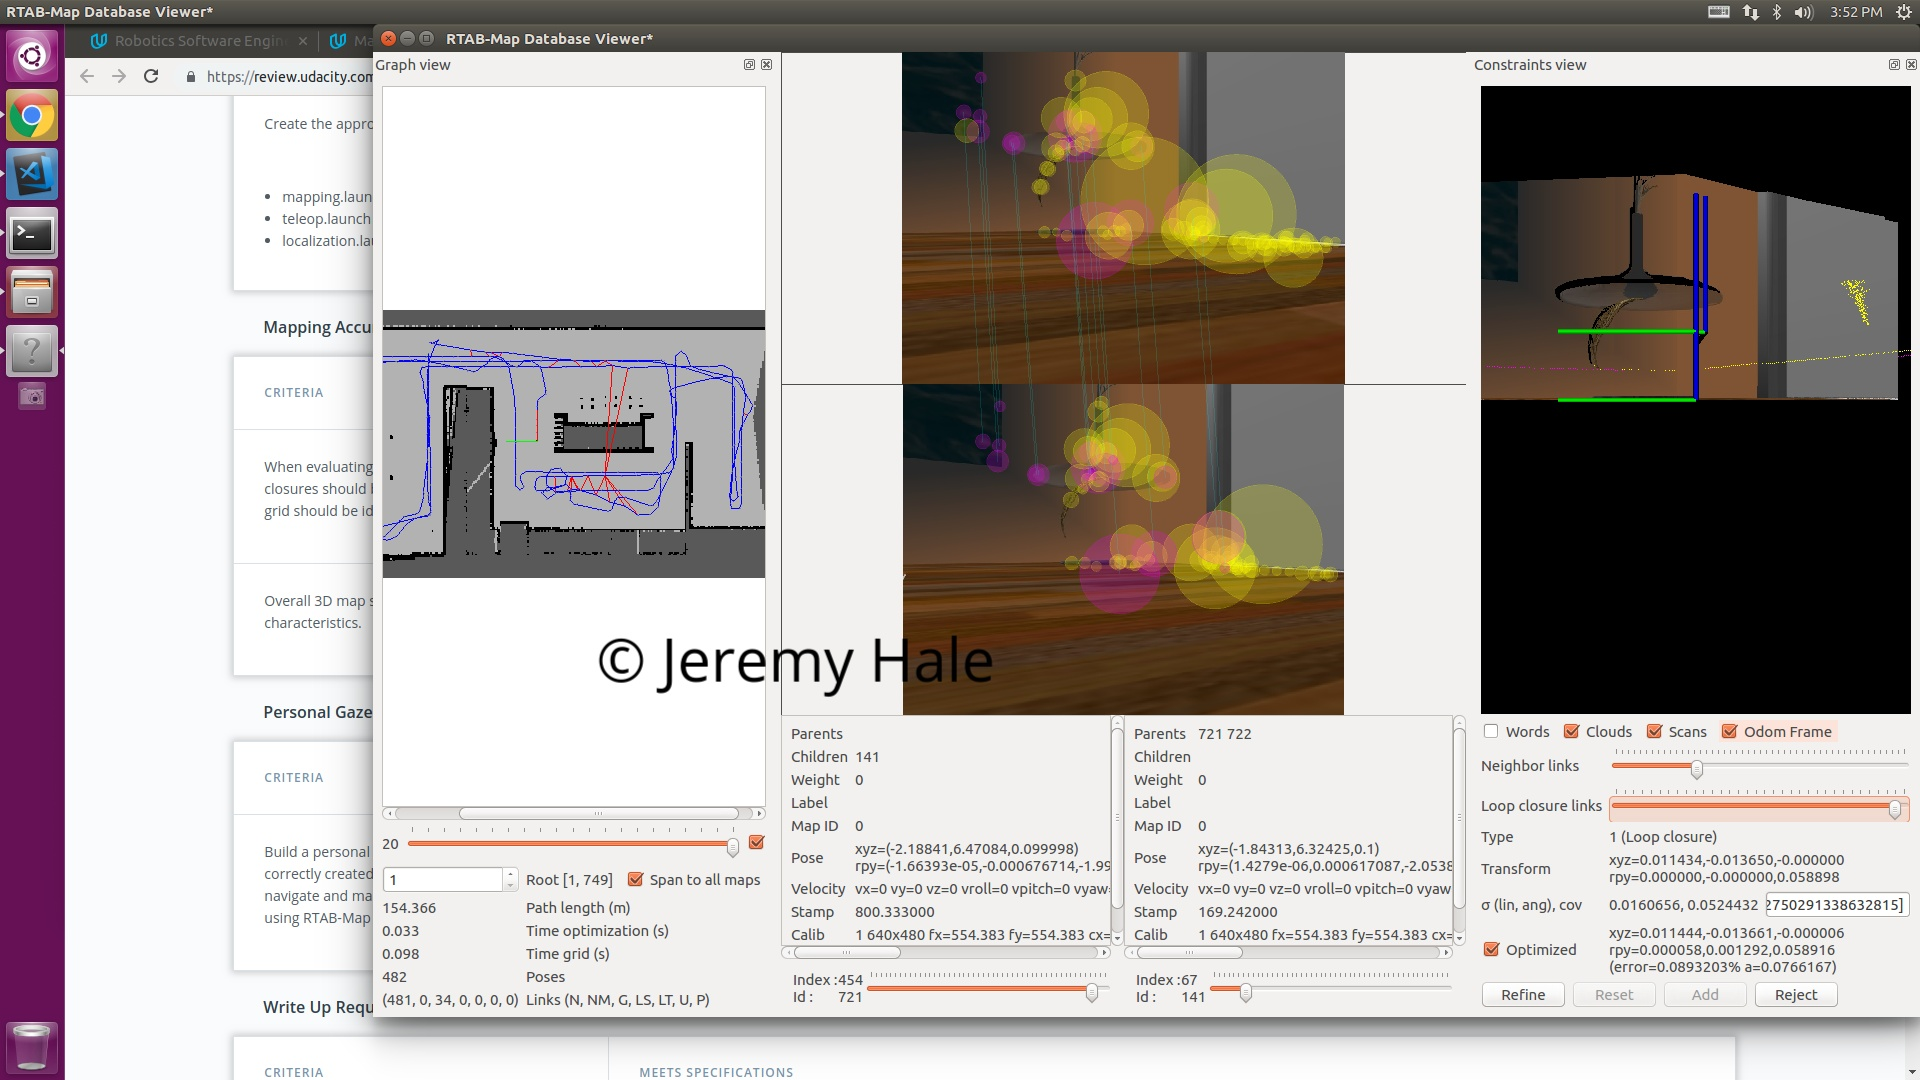
\includegraphics[width=\linewidth]{closure_3}
    \caption{Udacity World Closure}
    \label{fig:closure 3}
\end{figure}

\subsection{Back Alley}

The occupancy and 3D maps for the "Back Alley" world are shown below. There are also images showing the 3 closures.

\begin{figure}
    \centering
    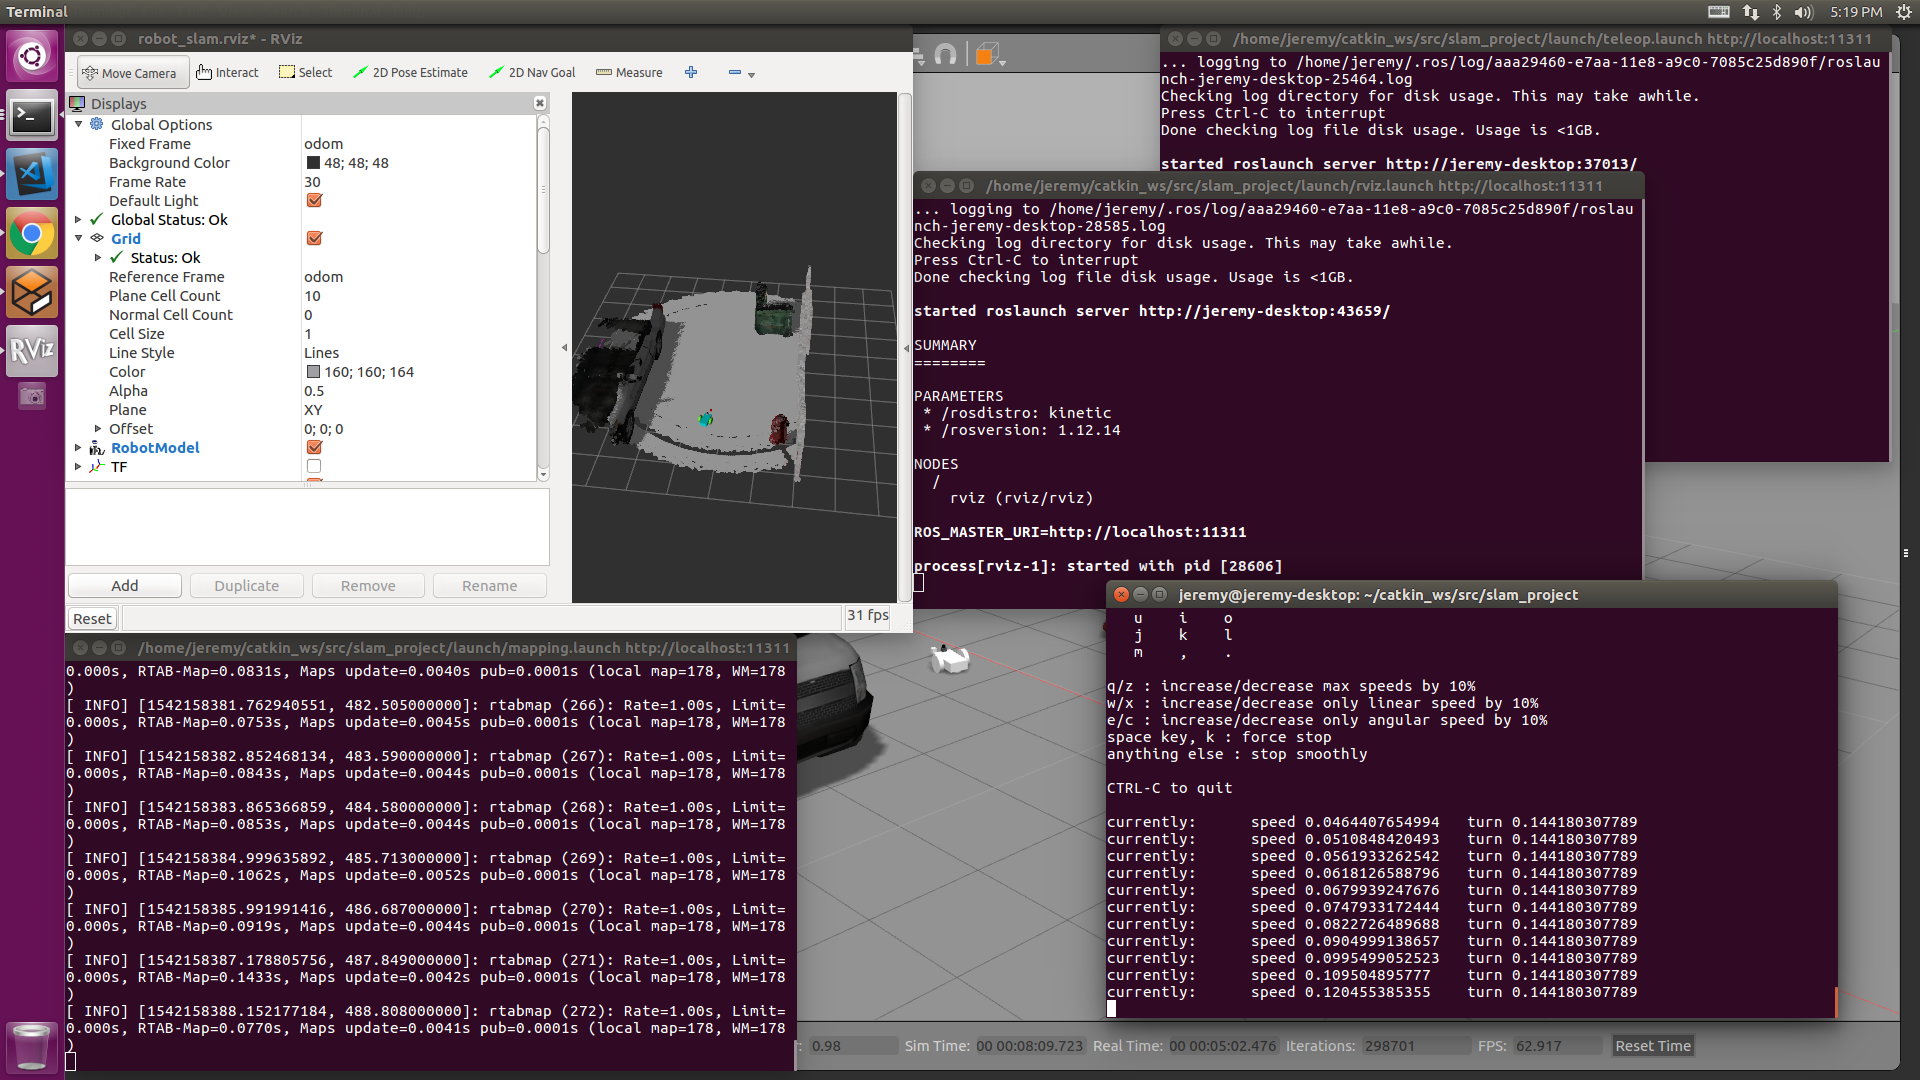
\includegraphics[width=\linewidth]{alley}
    \caption{Back Alley Process}
    \label{fig:alley_process}
\end{figure}

\begin{figure}
    \centering
    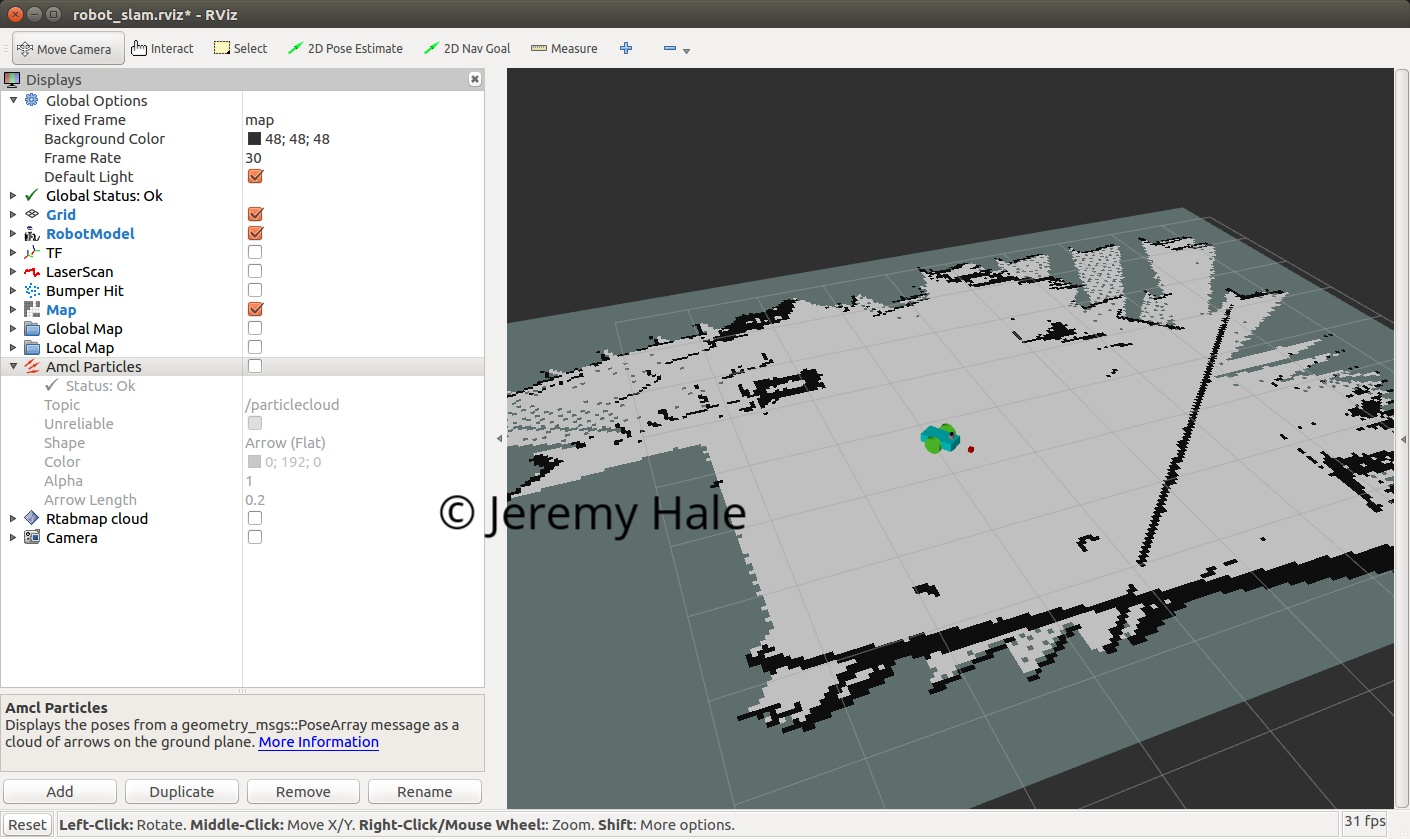
\includegraphics[width=\linewidth]{alley_occupancy}
    \caption{Back Alley Occupancy}
    \label{fig:alley_2d}
\end{figure}

\begin{figure}
    \centering
    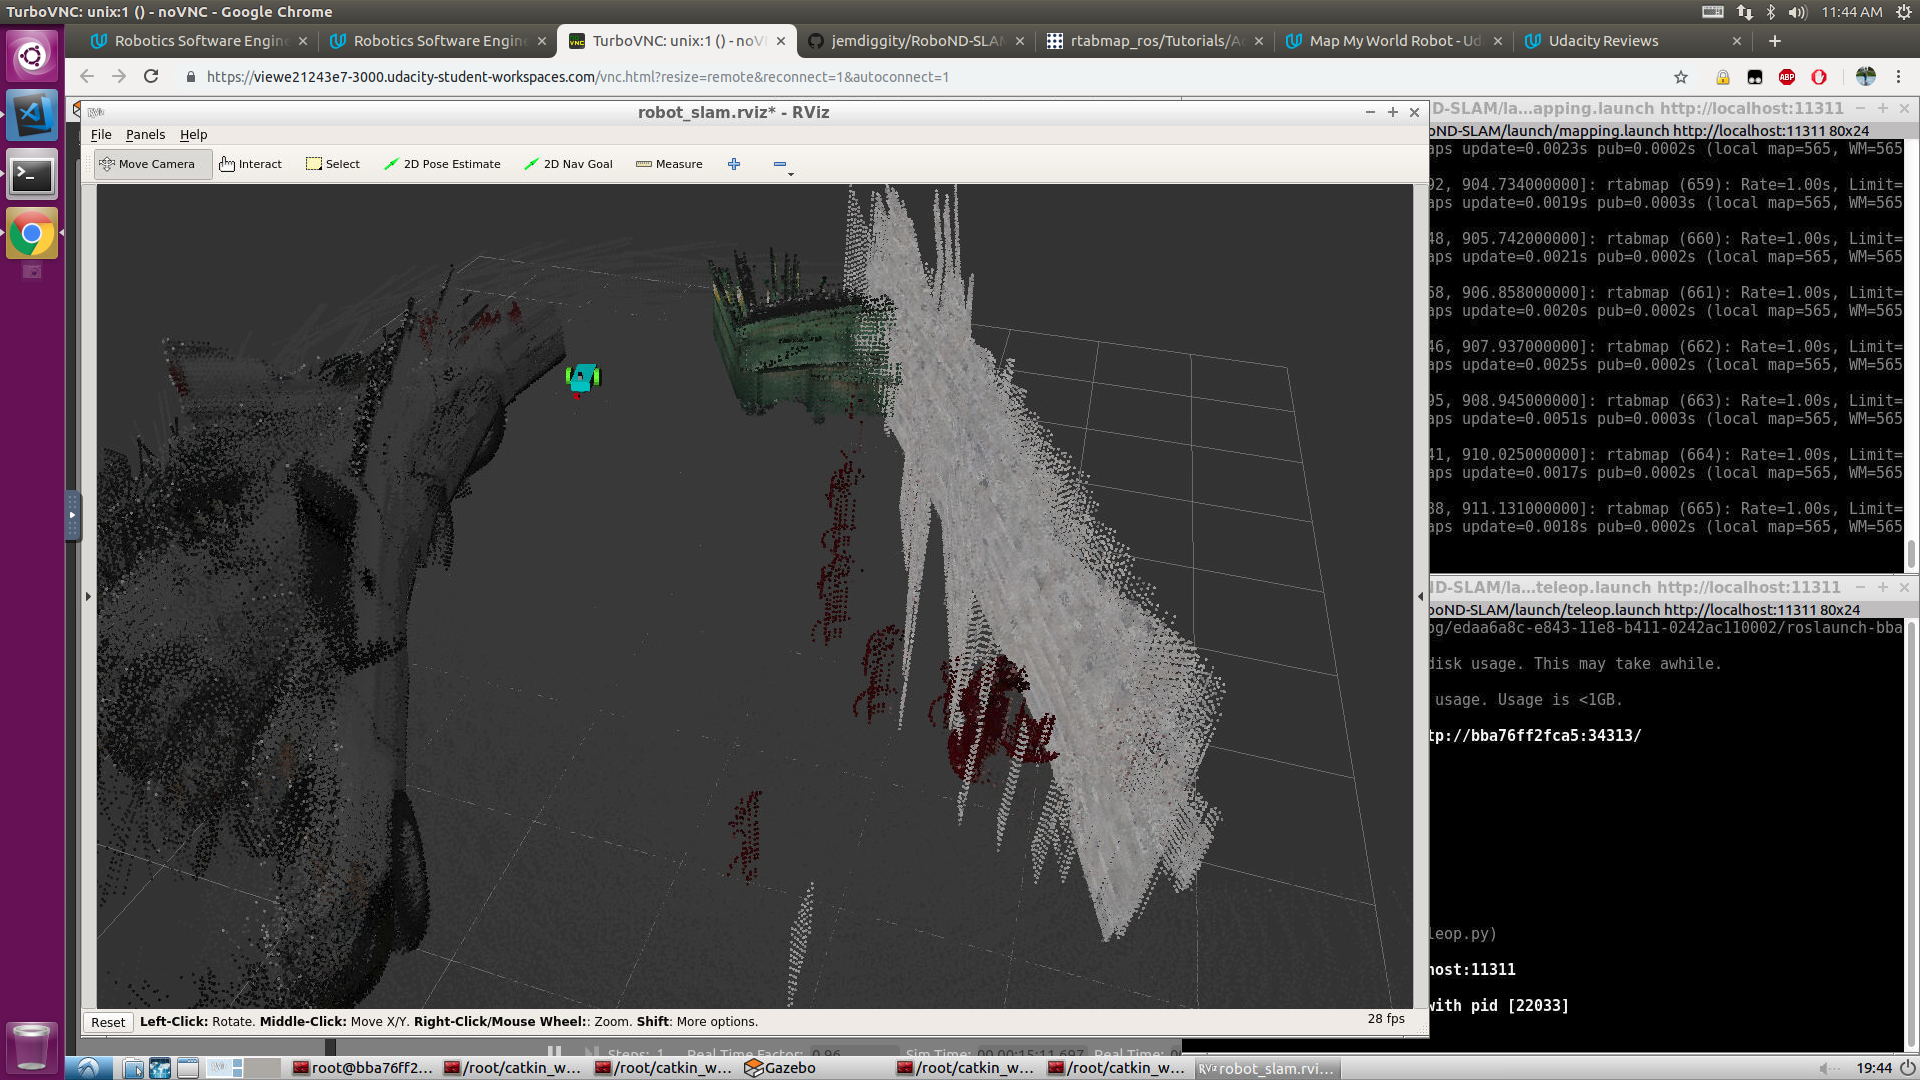
\includegraphics[width=\linewidth]{alley_confused}
    \caption{Back Alley Map}
    \label{fig:alley_3d}
\end{figure}

\begin{figure}
    \centering
    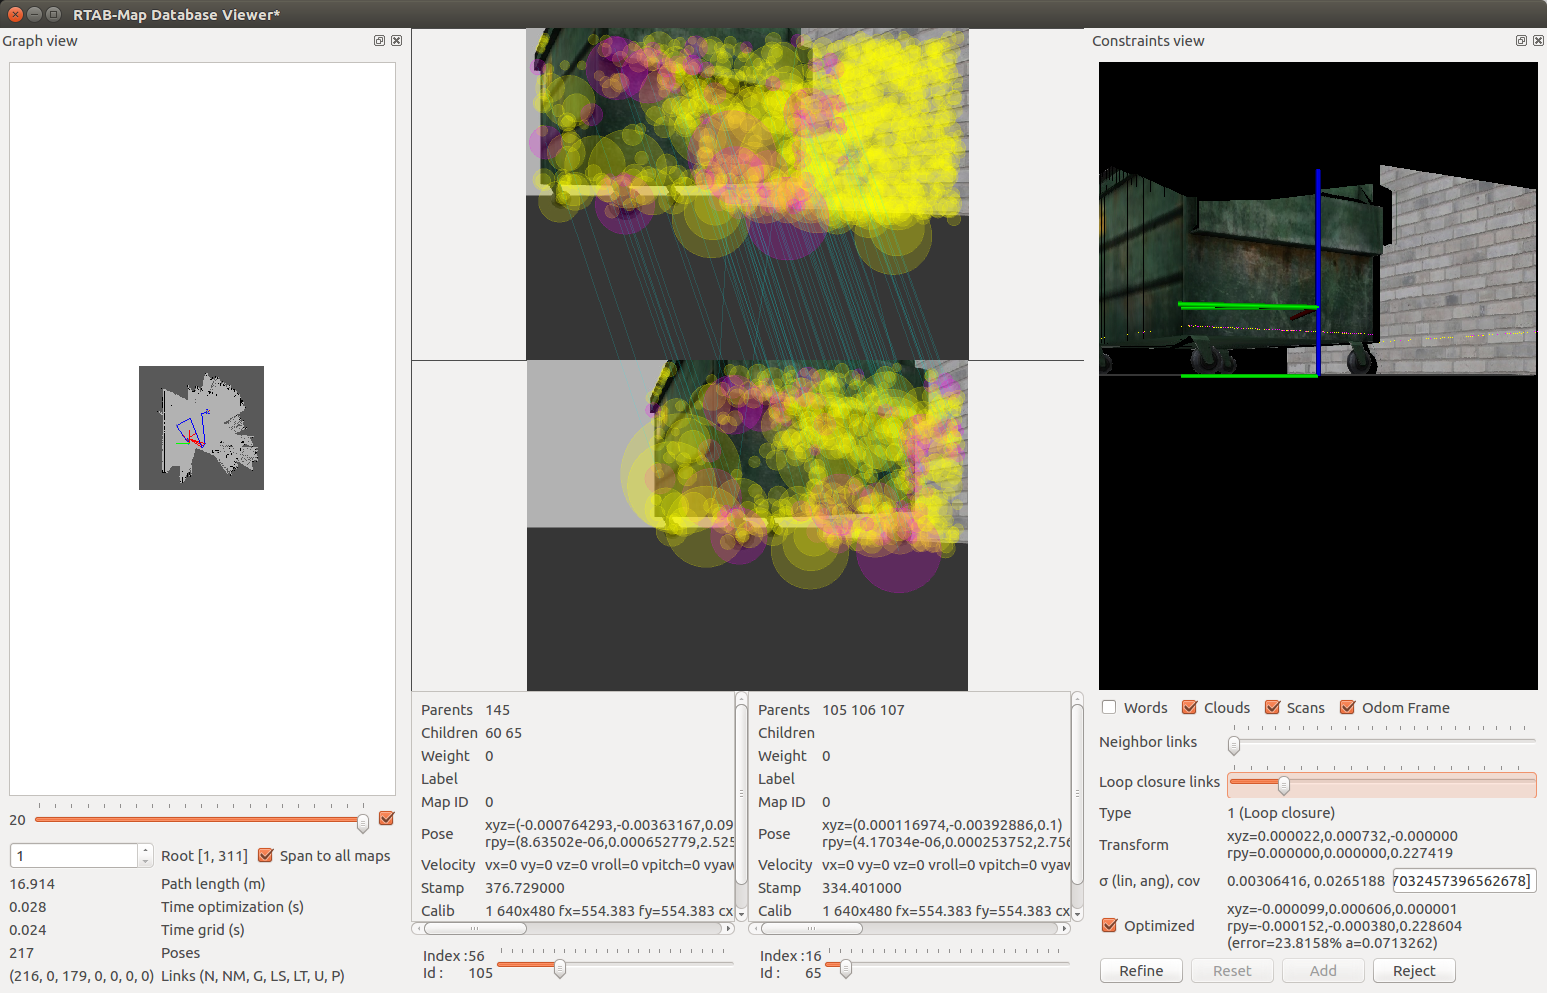
\includegraphics[width=\linewidth]{alley_closure_1}
    \caption{Alley Closure 1}
    \label{fig:alley_closure_1}
\end{figure}

\begin{figure}
    \centering
    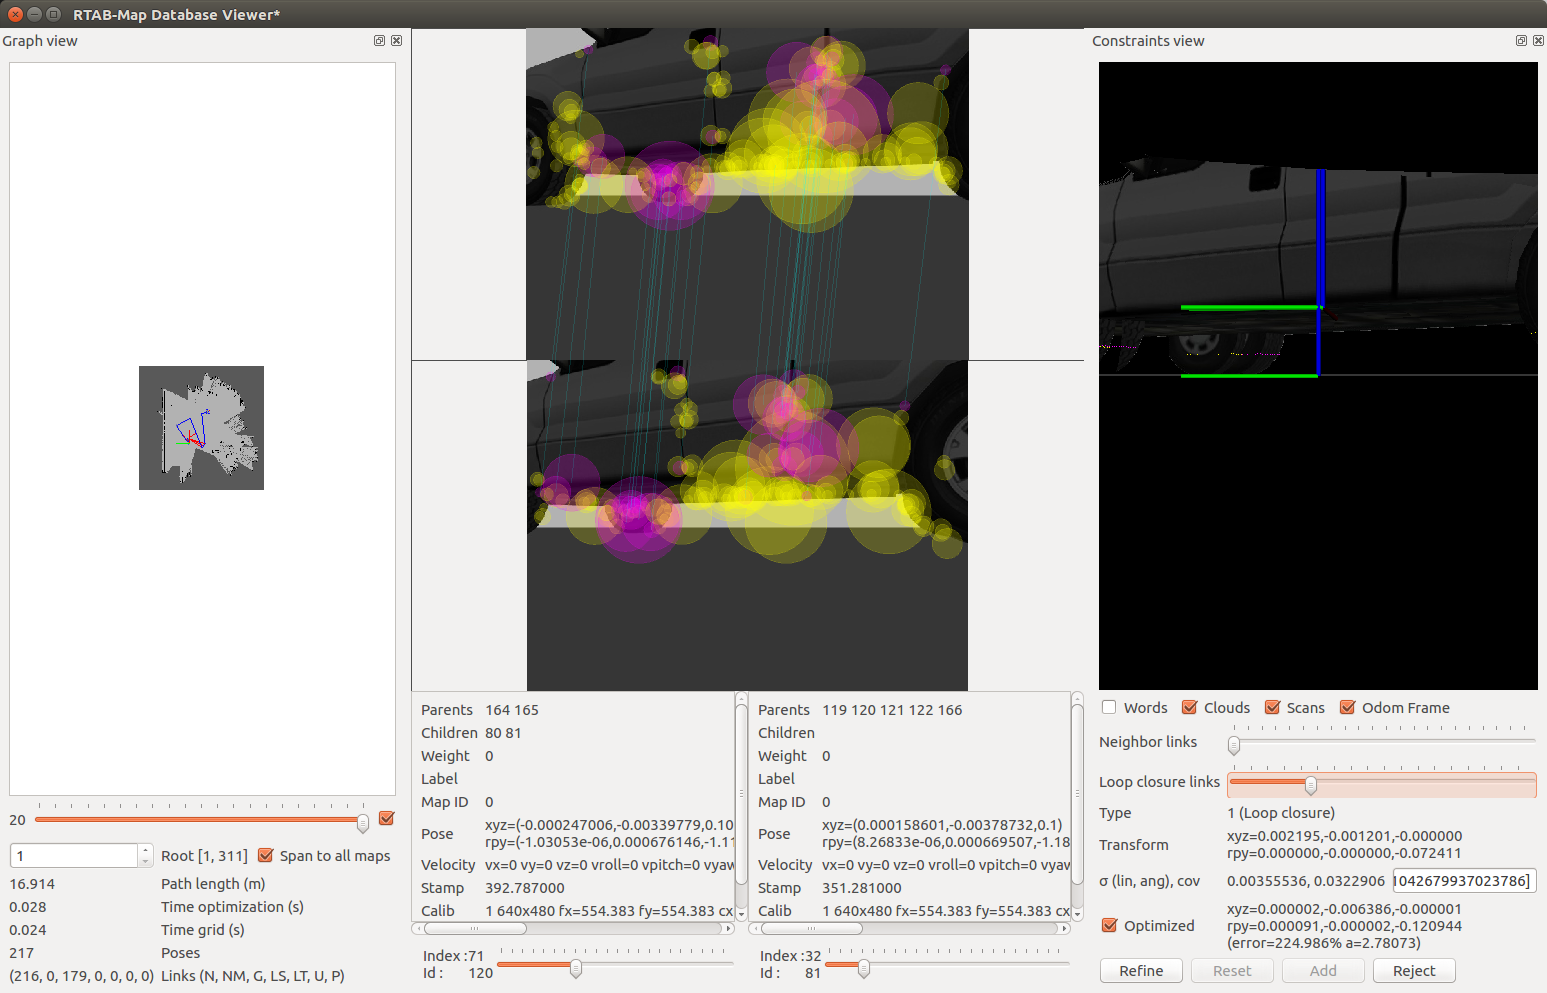
\includegraphics[width=\linewidth]{alley_closure_2}
    \caption{Alley Closure 2}
    \label{fig:alley_closure_2}
\end{figure}

\begin{figure}
    \centering
    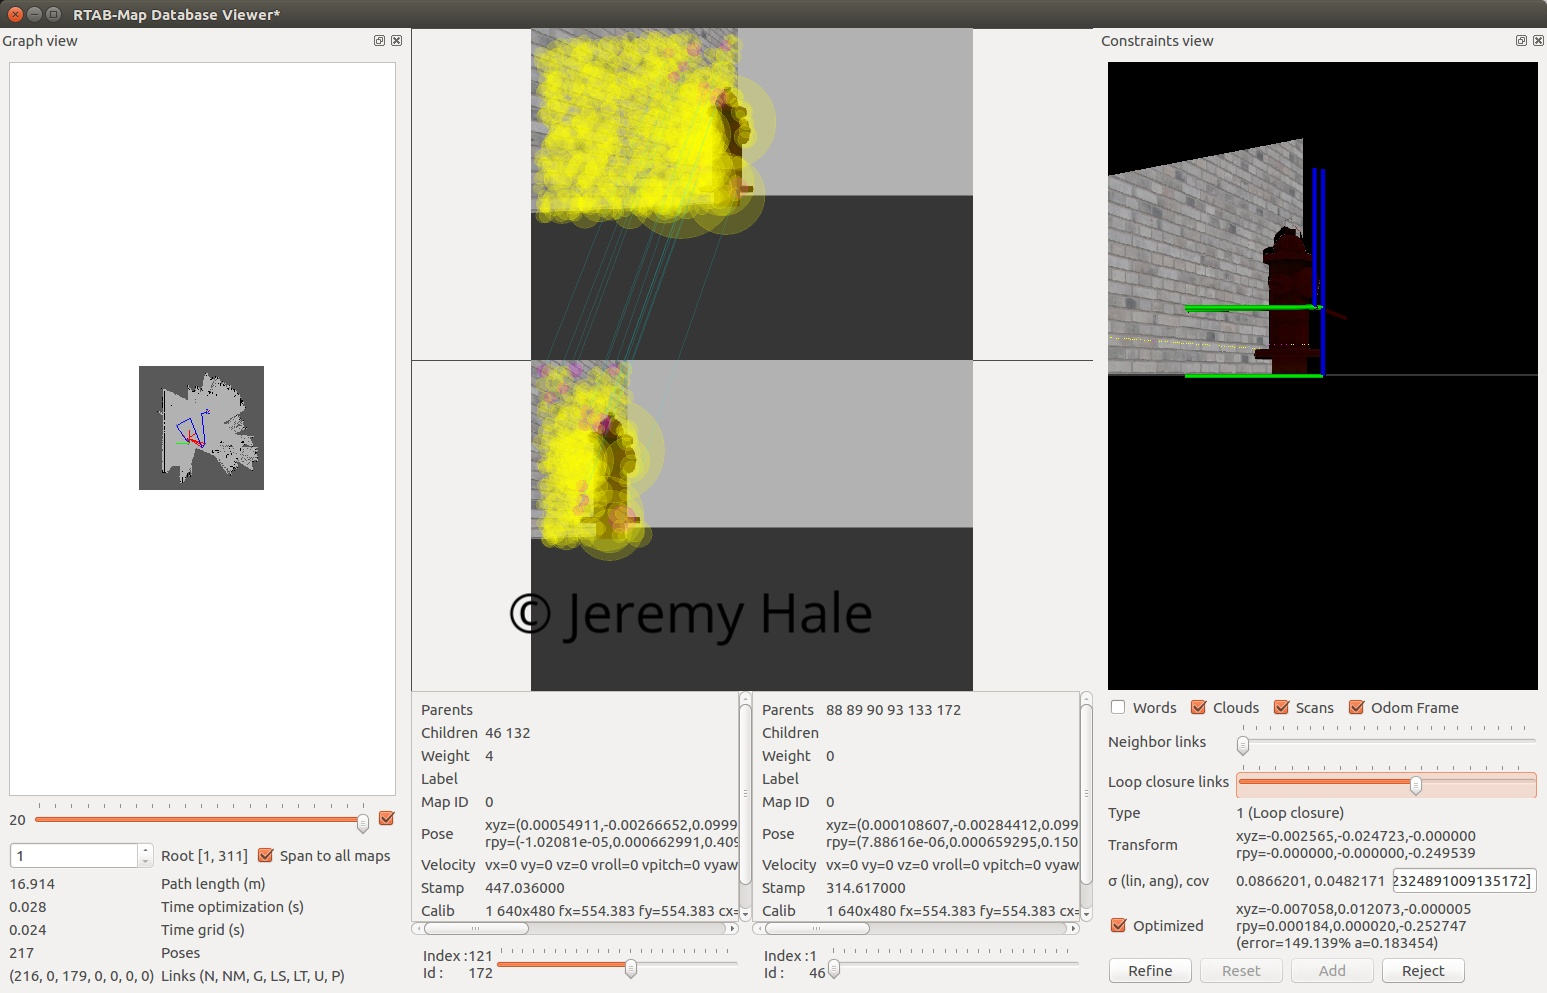
\includegraphics[width=\linewidth]{alley_closure_3}
    \caption{Alley Closure 3}
    \label{fig:alley_closure_3}
\end{figure}

\section{Discussion}
The mapping performance for the robot in the "Dining and Kitchen" world was satisfactory. Once the robot had re-traced its path, the RTAB-Map algorithm detected closures easily with subjectively little distortion.

Mapping the "Back Alley" world proved to be much more difficult. The mapping algorithm easily mixed up the rear and front wheel of the pickup truck causing mapping errors. A image from "rtabmap-databaseViewer" shows a closure between different truck wheels. Even with a bright orange traffic cone placed beside the wheel, the algorithm still had issues discerning the back and front wheels.

\begin{figure}
    \centering
    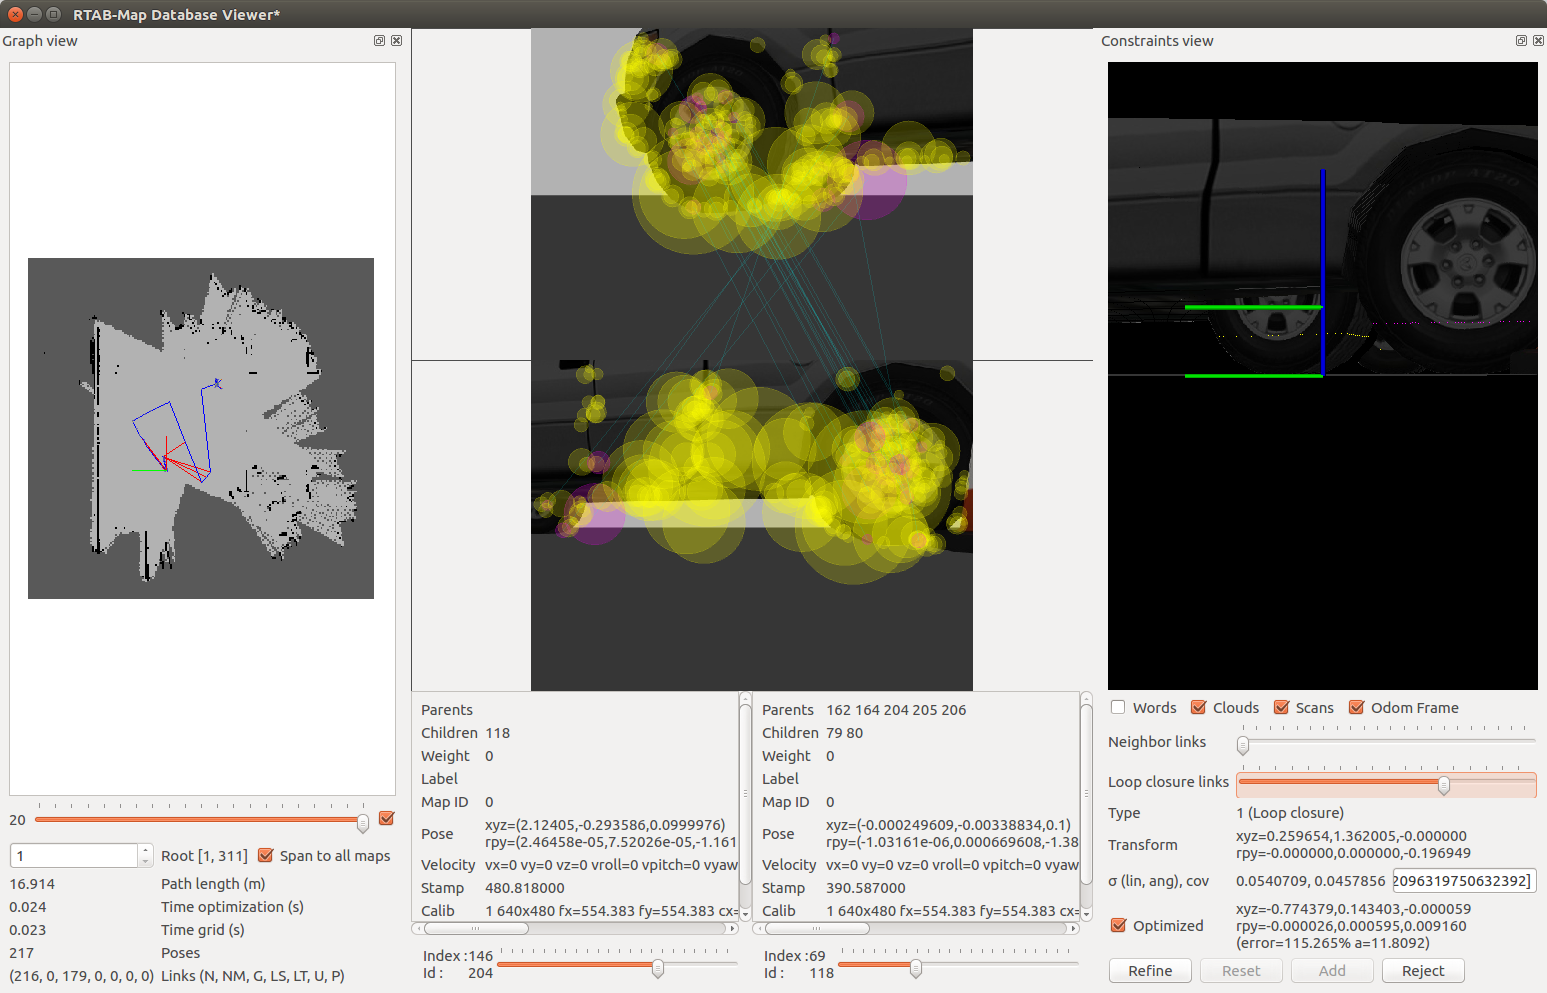
\includegraphics[width=\linewidth]{confused_cone_viewer}
    \caption{RTAB-Map Confused}
    \label{fig:confused}
\end{figure}

\begin{figure}
    \centering
    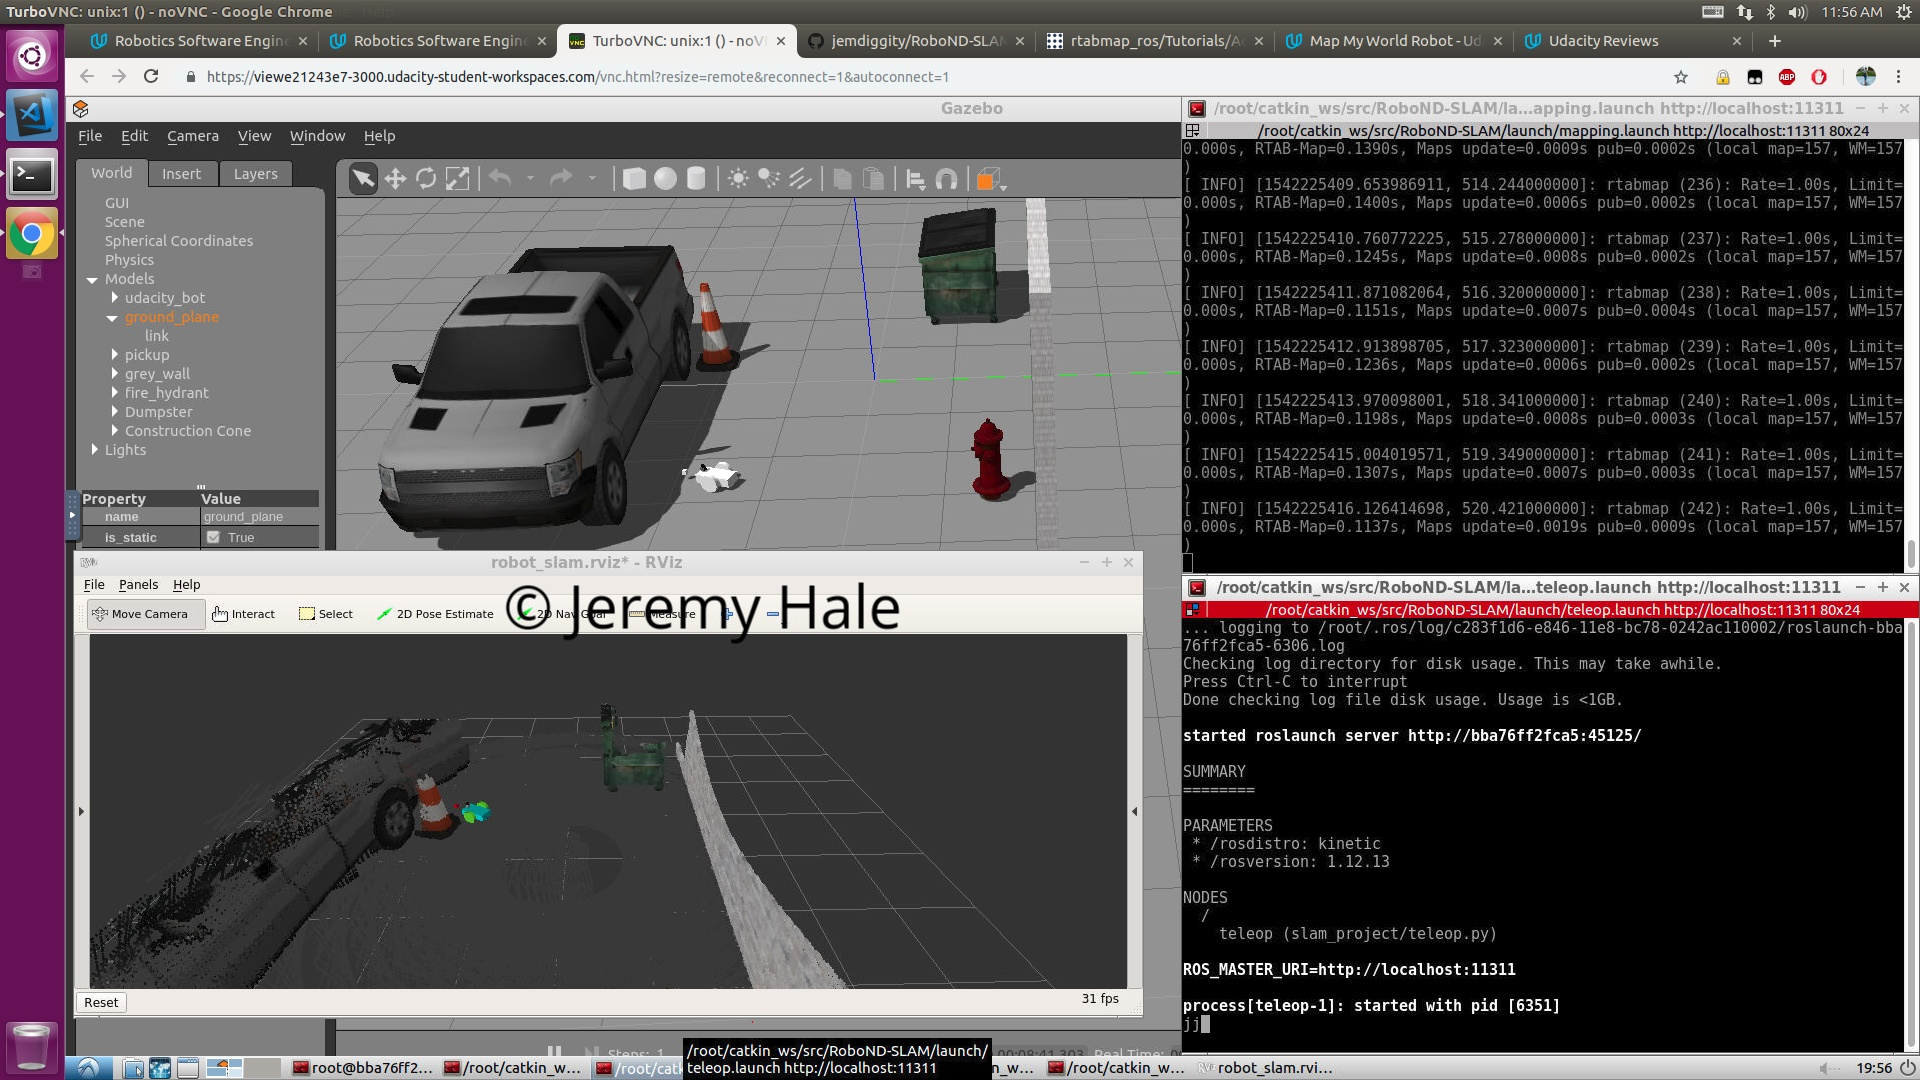
\includegraphics[width=\linewidth]{confused_cone}
    \caption{RTAB-Map Confused with Cone}
    \label{fig:confused_cone}
\end{figure}

Perhaps RTAB-Map can be tuned to have better performance. Adjusting the parameters for RTAB-Map was attempted as per the ROS RTAB-Map tutorial, but met limited success. There was also some confusion about setting up the ROS environment on a local machine and whether RTAB-Map 1.8 or 1.9 would work.

Navigating the small robot around was painfully slow. It took around 10 minutes to complete 3 circles of the environments.

\section{Conclusion / Future work}
Considering that the project was only a simulation of SLAM, it seems that it would be challenging to optimize and get satisfactory results in the real world. That being said, an interesting next step would be to model a real-life physical space, optimize parameters in simulation and then apply the same parameter tuning to the real-life space on a real-life robot such as the TurtleBot. The difference between simulation and real-life is always a challenge in engineering and a current area of research for deep reinforcement learning.

The RTAB-Map approach seems like it can work well for small indoor spaces. In an outdoor environment, the addition of existing maps and GPS may make SLAM unnecessary for solving the path planning problem, at least in a "global" sense, but SLAM may still be necessary for obstacle avoidance. Perhaps GPS information can be included along with LIDAR and RGBD data to improve results.

In future, to make simulation less time consuming and more practical, more automation is necessary. Manually navigating the robot in the environment is extremely time consuming. It would be much more efficient to predefine a path for the robot to follow and automate the teleoperation.

\end{document}
